\documentclass[review]{elsarticle}

\usepackage[margin=1in]{geometry}
\usepackage{hyperref}
\usepackage{subcaption}
%\usepackage{tabu}
\graphicspath{{./}{./figures/}{../figures/}}
\DeclareGraphicsExtensions{.pdf,.png,.jpg}
\usepackage{graphicx}
\usepackage{natbib}
\usepackage{amsmath}
\usepackage{lipsum}
\usepackage{lmodern}
\usepackage{tikz}
\usepackage{placeins}
\usetikzlibrary{shapes.geometric, arrows}
\usetikzlibrary{calc}
\tikzstyle{start} = [rectangle, rounded corners, minimum width=2cm, minimum height=1cm,text centered, text width=2cm, draw=black, fill=red!30]
\tikzstyle{io} = [trapezium, trapezium left angle=70, trapezium right angle=110, minimum width=3cm, text centered,text width = 4cm, minimum height=1cm, draw=black, fill=blue!30]
\tikzstyle{process} = [rectangle, minimum width=3cm, minimum height=1cm, text centered, draw=black, fill=orange!30]
\tikzstyle{decision} = [diamond, minimum width=3cm, minimum height=1cm, text centered, draw=black, text width=1.5cm,fill=green!30]
\tikzstyle{position} = [rectangle, minimum width=3cm, minimum height=1cm, text centered, draw=black,fill=blue!20]
\tikzstyle{arrow} = [thick,->,>=stealth]

\journal{Acta Materialia}
\bibliographystyle{elsarticle-num}

\begin{document}

\begin{frontmatter}

\title{Finite element analysis of plate--hole problem using FORTRAN90 code}
%\tnotetext[mytitlenote]{Fully documented templates are available in the elsarticle package on \href{http://www.ctan.org/tex-archive/macros/latex/contrib/elsarticle}{CTAN}.}

%% Group authors per affiliation:
\author{Srihari Sundar$^1$}
\address{$^1$Department of Metallurgical and Materials Engineering, Indian Institute of Technology Madras}

\begin{abstract}
A formula translator (FORTRAN) code is developed to perform finite element analysis (FEA) for the deformation of a 2D plate with a hole in the center. The results are compared with solution from ABAQUS. 
\end{abstract}

\begin{keyword}
FEM,FORTRAN,plate--hole,ABAQUS
\end{keyword}

\end{frontmatter}

%\section*{Introduction }

%\lipsum[1]

\section*{Flow of program}

\scalebox{0.8}{
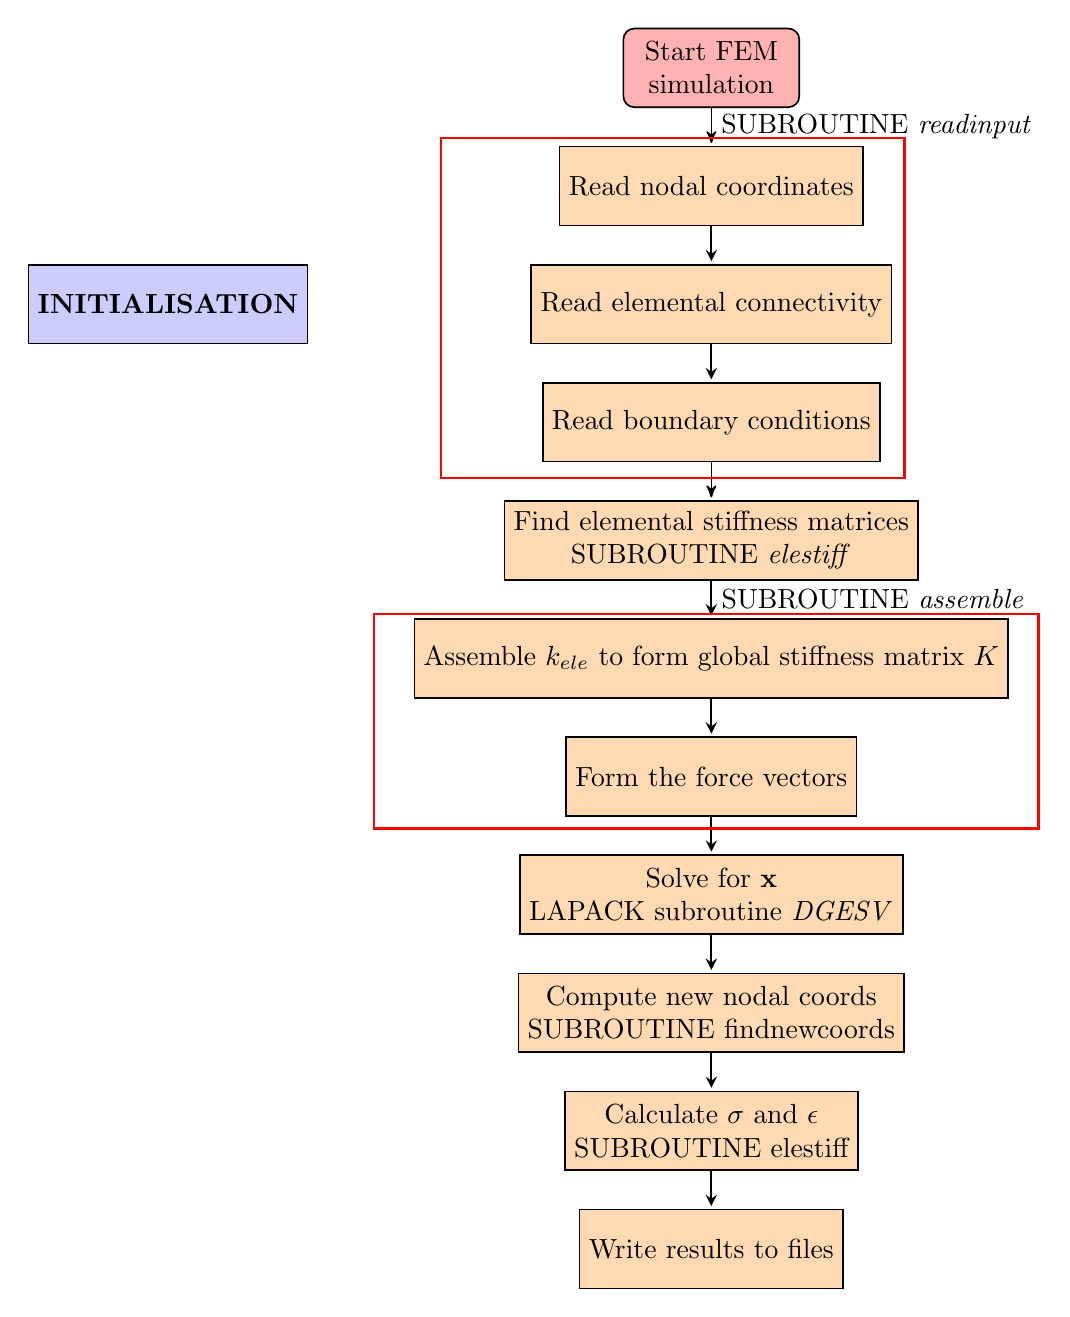
\begin{tikzpicture}[->,>=stealth',shorten >=1pt,auto,node distance=1.5cm,semithick]

\node (start) [start] {Start FEM simulation};
\node (readnode) [process,below of=start] {Read nodal coordinates};
\node (readele) [process,below of=readnode] {Read elemental connectivity};
\node (readbcs) [process,below of=readele] {Read boundary conditions};
\node (elestiff) [process,below of=readbcs,align=center] {Find elemental stiffness matrices \\ SUBROUTINE \emph{elestiff}};
\node (globalstiff) [process,below of=elestiff] {Assemble $k_{ele}$ to form global stiffness matrix $K$};
\node (formforce) [process,below of=globalstiff] {Form the force vectors};
\node (solve) [process,below of=formforce,align=center] {Solve for \textbf{x} \\ LAPACK subroutine \emph{DGESV}};
\node (newcoords) [process,below of=solve,align=center] {Compute new nodal coords \\ SUBROUTINE findnewcoords};
\node (strstr) [process,below of=newcoords, align=center] {Calculate $\sigma$ and $\epsilon$ \\ SUBROUTINE elestiff};
\node (results) [process,below of=strstr] {Write results to files};


\draw [->] (start) -- node{SUBROUTINE \emph{readinput}} (readnode);
\draw [arrow] (readnode) -- (readele);
\draw [arrow] (readele) -- (readbcs);
\draw [->] (readbcs) -- (elestiff);
\draw [arrow] (elestiff) -- node {SUBROUTINE \emph{assemble}} (globalstiff);
\draw [arrow] (globalstiff) -- (formforce);
\draw [arrow] (formforce) -- (solve);
\draw [arrow] (solve) -- (newcoords);
\draw [arrow] (newcoords) -- (strstr);
\draw [arrow] (strstr) -- (results);

\node (initialise) [position, left of=readele, xshift=-5.4cm] {\textbf{INITIALISATION}} ;

\draw[red,thick] ($(readnode.north west)+(-1.5,0.1)$)  rectangle ($(readbcs.south east)+(0.3,-0.2)$);
\draw[red,thick] ($(globalstiff.north west)+(-0.5,0.05)$)  rectangle ($(formforce.south east)+(2.3,-0.15)$);

\end{tikzpicture}
}

\newpage

\section*{Structure of input file}

1. nnodes,nelem

2. node numbers with nodal coordinates 

\hspace{3em}$\vdots$

3. elem numbers with nodes of element anti-clockwise direction starting from bottom left

\hspace{3em}$\vdots$

4. number of fixed nodes

5. node number, a,b (a,b=0--constrained,1-unconstrained)

6. number of nodes with force BC

7. node number,forceX,forceY

8. number of nodes with displacement BC
	
9. node number, dispX, dispY



\section*{Calculation of elemental stiffness matrix}
The element modeled here is a 4 noded element with 4 integration points \cite{entwistle1999basic}.

The interpolation functions used are as follows:

\[ N1={1\over4}(1-\xi)(1-\eta) \]
\[ N2={1\over4}(1+\xi)(1-\eta) \]
\[ N3={1\over4}(1+\xi)(1+\eta) \]
\[ N4={1\over4}(1-\xi)(1+\eta) \]

where $\xi$ and $\eta$ are the x and y coordinates in elemental reference frame. 

Over each integration point the following is carried out:

S and T are calculated which are $\xi$ and $\eta$ derivatives respectively. This is done in the subroutine \textit{\texttt{CALCULATE\_ST}}

\begin{minipage}{0.5\linewidth}
\begin{align*} 
S_1&=-{1\over4}(1-\eta) \\
S_2&={1\over4}(1-\eta) \\
S_3&={1\over4}(1+\eta) \\
S_4&=-{1\over4}(1+\eta) 
\end{align*}
\end{minipage}
\begin{minipage}{0.5\linewidth}
\begin{align*} 
T_1&=-{1\over4}(1-\xi) \\
T_2&=-{1\over4}(1+\xi) \\
T_3&={1\over4}(1+\xi) \\
T_4&={1\over4}(1-\xi) \\
\end{align*}
\end{minipage}
\bigskip

From these the `G' matrix is assembled as seen in fig. \ref{gmat}, in the subroutine \textit{\texttt{CALCULATE\_G}}.
\begin{figure}[ht!]
\centering
\includegraphics[width=0.9\textwidth]{gmat.png}
\caption{G matrix formulation}
\label{gmat}
\end{figure}

The `A' matrix is then calculated as seen in fig. \ref{amat}, in the subroutine \textit{\texttt{CALCULATE\_A}}.

\begin{figure}[ht!]
\begin{minipage}[b]{0.5\linewidth}
\centering
\includegraphics[width=0.8\textwidth]{amat.png}
\caption{`A' matrix formulation}
\label{amat}
\end{minipage}
\begin{minipage}[b]{0.5\linewidth}
\centering
\includegraphics[width=0.7\textwidth]{dmat.png}
\caption{Plane stress elasticity matrix}
\label{dmat}
\end{minipage}
\end{figure}

The Jacobians are calculated as:

\begin{minipage}{0.5\linewidth}
\centering
\[J_{11}=\sum_{i=1}^{8} s_i\times x_i\]
\[J_{21}=\sum_{i=1}^{8} t_i\times x_i\]
\end{minipage}
\begin{minipage}{0.5\linewidth}
\centering
\[J_{12}=\sum_{i=1}^{8} s_i\times y_i\]
\[J_{22}=\sum_{i=1}^{8} t_i\times y_i\]
\end{minipage}

where $x_{i}'s$ and $y_{i}'s$ are the coordinates of the nodes of the element in global frame. 

The following operations are then carried out succesively.

\[ [B]=[A][G] \]
\[ [C]=[D][B] \]
\[ [KI]=[B^T][C] \]

Based on displacements at the nodes the stress and strain are calculated as shown below.

\[ [\epsilon]=[B][du] \]
\[ [\sigma]=[D][d\epsilon] \]

Finally, the elemental stiffness matrix is calculated by:

\[ [K_{ele}]=[K_{ele}]+[KI]\times wt(ipt) \times detJ \]

The body forces are not presently considered.

The elemental stiffness matrices are assembled based on the nodal connectivity of each element and the boundary conditions to get the global elemental stiffness matrix. \cite{smith2005programming}

\section*{Simulation details}
The code is checked with test cases for deformation of a plate descritized with 1 element, 2 elements and 4 elements, and displacement boundary conditions. The input files and results are in the respective input and output files.

Then, a plate hole geometry is generated in ABAQUS \citep{abaqus} and the node and element information are ported into the input file for the FEM solver.

Details:

\begin{itemize}
\item Number of nodes : 454
\item Number of elements : 404
\item Plate size : 12*12
\item Bottom nodes are en-castrated
\item Top nodes are displaced in the y direction by +3 units
\end{itemize}

\section*{Results}

The x--displacement plots from ABAQUS \ref{u1_abq} as well as the FORTRAN code \ref{u1} show near matching qualitatively. Quantitatively, there is a small error of 3\%.
The same cannot be said about the y--displacement plots \ref{u2_abq} and \ref{u2}. Though the region wise there is a match of displacements, the contours are not properly seen, to be able to make better assessments.


\begin{figure}[ht!]
\centering
\includegraphics[width=0.9\textwidth]{u1_abq.png}
\caption{Displacement contour in x direction,ABAQUS}
\label{u1_abq}
\end{figure}

\begin{figure}[ht!]
\centering
\includegraphics[width=0.9\textwidth]{u11.png}
\caption{Displacement contour in x direction,FORTRAN code}
\label{u1}
\end{figure}

\begin{figure}[ht!]
\centering
\includegraphics[width=0.9\textwidth]{u2_abq.png}
\caption{Displacement contour in y direction,ABAQUS}
\label{u2_abq}
\end{figure}

\begin{figure}
\centering
\includegraphics[width=0.9\textwidth]{u21.png}
\caption{Displacement contour in y direction,FORTRAN code}
\label{u2}
\end{figure}

The stresses and strains at the integration points are also obtained, but these do not show sufficient agreement with the ABAQUS results.

\section*{References}
\bibliography{FEM_srihari}

\section*{Details of code}

Main file - 79 lines

Number of subroutines - 15

Functions file (Containing subroutines) - approximately 350 lines


\end{document}

